% ====================================
% DOCUMENT CLASS AND BASIC SETTINGS
% ====================================
\let\negmedspace\undefined
\let\negthickspace\undefined
\documentclass[journal]{IEEEtran}
\usepackage[a5paper, margin=10mm, onecolumn]{geometry}

% ====================================
% HEADER SETTINGS
% ====================================
\setlength{\headheight}{1cm}
\setlength{\headsep}{0mm}

% ====================================
% PACKAGE IMPORTS
% ====================================
% Custom packages
\usepackage{gvv-book}
\usepackage{gvv}
\usepackage{tfrupee}

% Math and symbols
\usepackage{amsmath,amssymb,amsfonts,amsthm}
\usepackage{mathtools}
\usepackage{gensymb}

% Tables, graphics, and colors
\usepackage{graphicx}
\usepackage{xcolor}
\usepackage{array}
\usepackage{longtable}
\usepackage{multirow}
\usepackage{hhline}
\usepackage{calc}
\usepackage{lscape}

% Text formatting and listings
\usepackage{textcomp}
\usepackage{txfonts}
\usepackage{listings}
\usepackage{algorithmic}
\usepackage{enumitem}
\usepackage{comment}
\usepackage{cite}

% Drawing
\usepackage{tkz-euclide}

% Input encoding
\usepackage[latin1]{inputenc}

% Hyperlinks
\usepackage[breaklinks=true]{hyperref}

% Define input for gnumeric table
\def\inputGnumericTable{}


\title{\textbf{Hardware Project - Digital Clock}}
\author{EE24BTECH11012 - Bhavanisankar G S}
\date{\today}

\begin{document}

\maketitle
\thispagestyle{empty}

\tableofcontents

\bigspace
% ====================================
% NUMBERING SETTINGS
% ====================================
\renewcommand{\thefigure}{\theenumi}
\renewcommand{\thetable}{\theenumi}
\setlength{\intextsep}{10pt} % Space between text and floats
\numberwithin{equation}{enumi}
\numberwithin{figure}{enumi}
\renewcommand{\thetable}{\theenumi}

% ====================================
% ABSTRACT
% ====================================
\begin{abstract}
\begin{enumerate}
    \item This report presents the design and implementation of a digital clock using a 7-segment display and a microcontroller. The system employs a multiplexing technique to efficiently control six 7-segment displays, representing HH:MM:SS format. A BCD to 7-segment decoder is used to reduce the number of required microcontroller pins while ensuring accurate digit representation. The timekeeping functionality is implemented through internal software logic, handling the increment of seconds, minutes, and hours.
    \item User interaction is facilitated via push buttons, allowing for time adjustments and mode selection between Clock, Timer, and Stopwatch functionalities. The system ensures stable and precise operation through effective debouncing, power management, and signal stability techniques.
    \end{enumerate}
\end{abstract}

% ====================================
% INTRODUCTION
% ====================================
\section{Introduction}
\begin{enumerate}
\item A digital clock is an essential timekeeping device used in various applications, from household appliances to industrial systems. Unlike analog clocks, digital clocks display time numerically, making them easy to read and interpret. This project aims to design and implement a digital clock using an Arduino UNO microcontroller, 7-segment displays, and the IC 7447 BCD to 7-segment decoder. The Arduino serves as the brain of the clock, handling timekeeping and display multiplexing, while the IC 7447 simplifies the connection between the microcontroller and the 7-segment display by converting binary-coded decimal (BCD) signals into 7-segment outputs.
\item The clock will consist of six 7-segment displays, representing hours, minutes, and seconds. It will also include push buttons to set the time manually. By implementing display multiplexing, the circuit efficiently controls all six digits using minimal Arduino pins.
\item Multiplexing enhances the modularity of the setup by reducing the number of decoders from 6 ( one per display ) to 1 by keeping a very small delay and exploiting the persistence of vision of human eye.
\end{enumerate}

% ====================================
% COMPONENTS USED
% ====================================
\section{Components Used}
\begin{table}[H]
    \centering
    \renewcommand{\arraystretch}{1.2} % Adjust row height
    \begin{tabular}{|p{4cm}|p{5cm}|p{2cm}|}
        \hline
        \textbf{Component} & \textbf{Specification / Purpose} & \textbf{Quantity} \\
        \hline
        \textbf{Microcontroller} & Arduino (Uno/Nano/Mega) - Controls timekeeping and display multiplexing & 1 \\
        \hline
        \textbf{7-Segment Display} & Common Anode - Displays hours, minutes, and seconds & 6 \\
        \hline
        \textbf{IC 7447} & BCD to 7-segment decoder - Converts BCD input to 7-segment output & 3 \\
        \hline
        \textbf{Push Buttons} & Used for setting and adjusting time & 4+ \\
        \hline
        \textbf{Resistors} &  330$\Omega$ (current limiting) & Multiple \\
        \hline
        \textbf{Power Supply} & 5V (USB or adapter) - Powers the circuit & 1 \\
        \hline
        \textbf{Breadboard} & Used for prototyping the circuit & 1 \\
        \hline
        \textbf{Connecting Wires} & Used to connect components & As needed \\
        \hline
    \end{tabular}
    \caption{List of Components Used in the Digital Clock Project}
    \label{tab:components}
\end{table}

% ====================================
% CLOCK DISPLAY AND CONNECTIONS
% ====================================
\section{Clock Display and Connections}

The clock is designed using six 7-segment displays to represent the time in the \textbf{HH:MM:SS} format. The display is controlled using an \textbf{Arduino}, a \textbf{7447 BCD to 7-segment decoder}, and a multiplexing technique to minimize pin usage.

\subsection{Connections}
\begin{figure*}[!htb]
    {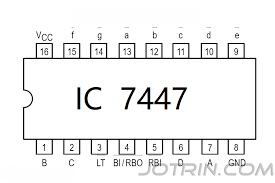
\includegraphics[ width=0.31\textwidth]{figs/7447.png}}
    \hspace{\fill}
    {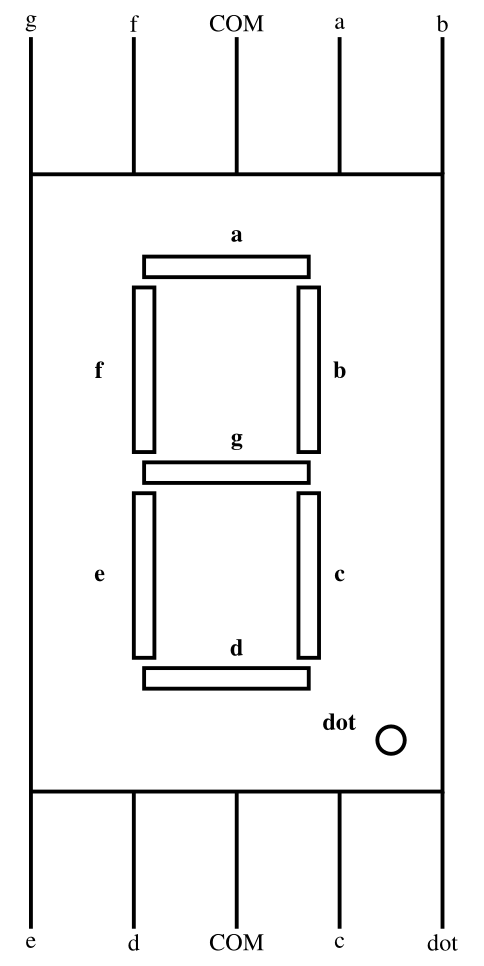
\includegraphics[ width=0.31\textwidth]{figs/ssd.png}}
    \hspace{\fill}
\end{figure*}

\begin{figure}[H]
	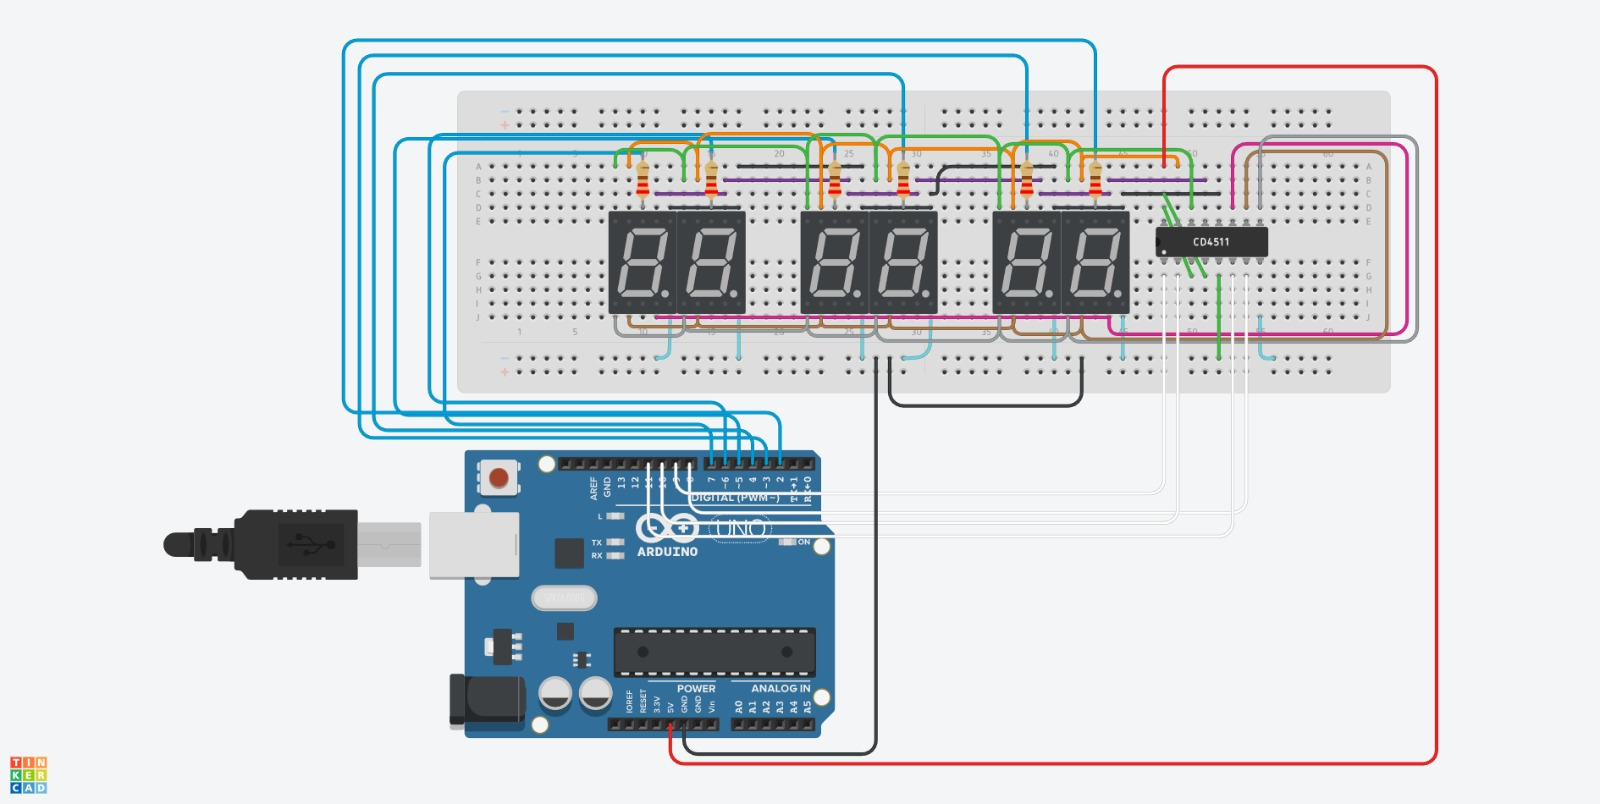
\includegraphics[width=\columnwidth]{figs/schematic.jpg}
	\caption{Schematic sketch}
	\label{Schematic}
\end{figure}

\subsubsection{Interface Between Arduino and 7447 IC}
\begin{enumerate}
    \item The \textbf{Arduino} provides \textbf{4-bit Binary-Coded Decimal (BCD)} signals (\texttt{A, B, C, D}) as input to the \textbf{7447 BCD to 7-segment decoder IC}.
    \item The \textbf{7447 decoder} converts the BCD input into corresponding \textbf{7-segment outputs} (\texttt{a, b, c, d, e, f, g}) to illuminate the appropriate segments.
    \item This setup allows the display of decimal digits (0-9) on the 7-segment display.
\end{enumerate}

\subsubsection{Multiplexing and Common Anode Control}
\begin{enumerate}
    \item The \textbf{six 7-segment displays} share a common set of segment control lines (\texttt{a--g}).
    \item The anode terminals of the displays are controlled using \textbf{multiplexing}, allowing only one display to be active at a time.
    \item The Arduino rapidly cycles through the digit enable lines, making all displays appear \textbf{continuously ON} due to \textbf{persistence of vision}.
    \item This technique significantly reduces the number of required Arduino pins.
\end{enumerate}

\subsubsection{Push Button Controls}
The clock includes push-button switches for user interaction. These buttons enable manual control of time settings and clock modes.

\begin{itemize}
    \item \textbf{Hour Increment Button}: Increases the hour value.
    \item \textbf{Minute Increment Button}: Increases the minute value.
    \item \textbf{Second Increment Button}: Increases the second value.
    \item \textbf{Mode Selection Button}: Toggles between \textbf{Clock}, \textbf{Timer}, and \textbf{Stopwatch} modes.
    \item \textbf{Timer Control Button}: Starts, stops, or resets the timer function.
\end{itemize}

% ====================================
% WORKING PRINCIPLE
% ====================================
\section{Working Principle}

The clock operates by displaying time in the format \textbf{HH:MM:SS} using six \textbf{7-segment displays}. To efficiently control the displays while minimizing the number of required Arduino pins, a \textbf{multiplexing technique} is employed. The 7447 BCD to 7-segment decoder converts binary-coded decimal (BCD) inputs into corresponding 7-segment outputs. The system also incorporates push-button inputs for adjusting time and toggling clock modes.

\subsection{Time Representation and Display Mechanism}

\begin{itemize}
    \item The six 7-segment displays are arranged to show hours, minutes, and seconds.
    \item Since the Arduino has a limited number of GPIO pins, it does not directly control each segment of all six displays.
    \item Instead, it sends a \textbf{4-bit BCD value} (A, B, C, D) to a \textbf{7447 decoder}, which translates it into segment activation signals (\texttt{a--g}).
    \item The decoder drives the individual segments of the 7-segment displays.
\end{itemize}

\subsection{Multiplexing Technique for Display Control}

\begin{itemize}
    \item Problem: Controlling all six displays simultaneously would require a large number of Arduino pins.
    \item Solution: A \textbf{multiplexing} approach is used where only one display is activated at a time.
    \item How it Works:
    \begin{enumerate}
        \item The Arduino sends the BCD values for a digit to the 7447 decoder.
        \item The Arduino enables one display at a time by controlling the common anode lines.
        \item The Arduino then quickly cycles through all six displays, activating one at a time.
        \item Because this switching happens rapidly (typically in milliseconds), the human eye perceives all displays as being ON simultaneously due to \textbf{persistence of vision}.
    \end{enumerate}
    \item This approach drastically reduces the number of required Arduino pins while still displaying six digits.
\end{itemize}

\subsection{Timekeeping Mechanism}

\begin{itemize}
    \item The Arduino maintains a time count internally, incrementing seconds every 1000 milliseconds. This is done by incorporating the Boolean logic of addition.
    \item Since, the numbers we display are from 0 to 9, which can be represented with the help of four bits, the code uses the binary logic of addition of four bit numbers. The corresponding truth table for addition is given below.
    \begin{table}[H]
    \centering
    \renewcommand{\arraystretch}{1.3}
    \begin{tabular}{|c c c c|c|c c c c|c|}
        \hline
        \multicolumn{4}{|c|}{\textbf{BCD Input (A B C D)}} & \textbf{Value} & \multicolumn{4}{c|}{\textbf{BCD Output (W X Y Z)}} & \textbf{Value} \\
        \hline
        A & B & C & D & Dec & W & X & Y & Z & Dec \\
        \hline
        0 & 0 & 0 & 0 & 0  & 0 & 0 & 0 & 1 & 1  \\
        0 & 0 & 0 & 1 & 1  & 0 & 0 & 1 & 0 & 2  \\
        0 & 0 & 1 & 0 & 2  & 0 & 0 & 1 & 1 & 3  \\
        0 & 0 & 1 & 1 & 3  & 0 & 1 & 0 & 0 & 4  \\
        0 & 1 & 0 & 0 & 4  & 0 & 1 & 0 & 1 & 5  \\
        0 & 1 & 0 & 1 & 5  & 0 & 1 & 1 & 0 & 6  \\
        0 & 1 & 1 & 0 & 6  & 0 & 1 & 1 & 1 & 7  \\
        0 & 1 & 1 & 1 & 7  & 1 & 0 & 0 & 0 & 8  \\
        1 & 0 & 0 & 0 & 8  & 1 & 0 & 0 & 1 & 9  \\
        1 & 0 & 0 & 1 & 9  & 0 & 0 & 0 & 0 & 0  \\
        \hline
    \end{tabular}
    \caption{Truth Table for BCD Increment by One}
\end{table}
    \item The logic can be seen as - \\
    A = !W  \\
    B = (!W && X) $||$ (W && !X && !Z)  \\
    C = (!X && Y) $||$ (!W && Y) $||$ (W && X && !Y)  \\
    D = (!W && Z) $||$ (W && X && Y)  \\
    \item The system keeps track of time using a software counter:
    \begin{enumerate}
        \item Every 1000ms, the seconds counter increments.
        \item When seconds reach \textbf{60}, they reset to \textbf{00}, and minutes increment by \textbf{1}.
        \item When minutes reach \textbf{60}, they reset to \textbf{00}, and hours increment by \textbf{1}.
        \item When hours reach \textbf{24}, they reset to \textbf{00}.
    \end{enumerate}
\end{itemize}

\subsection{Push Button Functionality}

To allow user interaction, several push-button inputs are integrated:

\begin{itemize}
    \item \textbf{Increment Hours Button}: Adds 1 to the hour value (rolls over after 23).
    \item \textbf{Increment Minutes Button}: Adds 1 to the minute value (rolls over after 59).
    \item \textbf{Increment Seconds Button}: Adds 1 to the second value (for manual adjustment).
    \item \textbf{Mode Toggle Button}: Cycles between Clock, Timer, and Stopwatch modes.
    \item \textbf{Timer Control Button}: Starts, stops, or resets the timer in Timer Mode.
\end{itemize}

\subsection{Power Management and Efficiency}

\begin{itemize}
    \item Since only one display is lit at a time, power consumption is reduced.
    \item The multiplexing technique optimizes pin usage and efficiency.
    \item The system can be powered via USB (5V) or an external power source.
\end{itemize}

% ====================================
% CONCLUSION
% ====================================
\section{Conclusion}
\begin{enumerate}
\item This project successfully demonstrates the design and implementation of a digital clock using an Arduino, 7-segment displays, and the 7447 BCD to 7-segment decoder. By employing multiplexing, the system efficiently controls six displays while minimizing the number of required microcontroller pins. The timekeeping mechanism is implemented through software, ensuring accurate second, minute, and hour updates.
\item Additionally, user interaction is facilitated through push-button inputs, allowing manual time adjustments and mode selection between Clock, Timer, and Stopwatch functionalities. The system effectively handles power consumption by enabling only one display at a time, reducing overall energy usage.
\item The corresponding codes can be seen here - \href{https://github.com/EE24BTECH11012/EE1003/tree/c55818859eebe407cd8a028f4a39012ec59f1942/Hardware/Clock-final}{https://github.com/EE24BTECH11012/EE1003/Hardware/Clock-final}
\end{enumerate}
\end{document}
